\subsection{Timer interrupts}
\label{sec:libinger:signals}

\begin{figure}
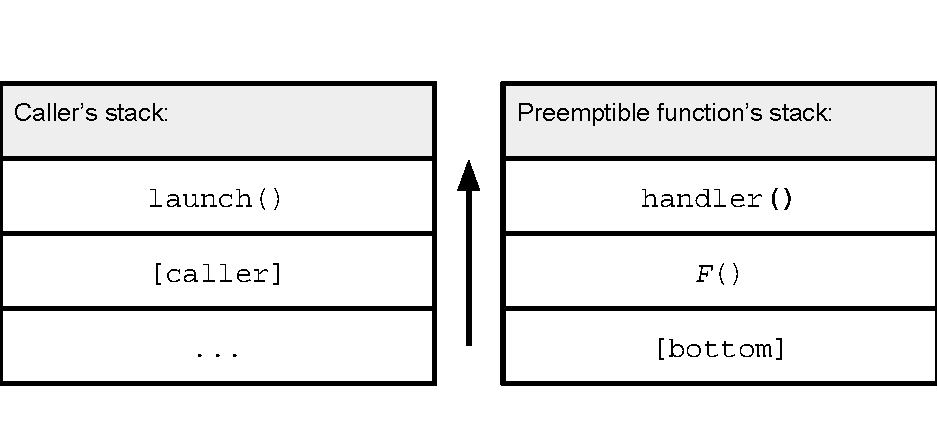
\includegraphics[width=\columnwidth]{figs/twostacks}
\caption{The stacks just before a timeout.  \textnormal{Upon discovering
that the preemptible function has exceeded its time bound, the handler jumps into the
\texttt{launch()} (or \texttt{resume()}) function, which in turn returns to the
original call site, removing its own stack frame in the process.}}
\label{fig:twostacks}
\end{figure}

Whenever \textit{libinger} is executing a user-provided function, we
enable fine-grained timer interrupts to
monitor that function's elapsed running time.  A timer interrupt fires
periodically,\footnote{Signal arrival is accurate to microsecond timescales, but
exhibits a warmup effect.  For simplicity, we use a fixed signal frequency for all
preemptible functions, but this is not fundamental to the design.  In the future,
we plan to adjust each function's frequency based on its timeout, and to delay the
first signal until shortly before the prescribed timeout (in the case of
longer-running functions).} causing our signal
handler to be invoked.  If the function exceeds its timeout,
this handler saves a continuation by dumping the machine's registers.  It then
performs an unstructured jump out of the signal handler and back into the
\texttt{launch()} or \texttt{resume()} function, switching back to the caller's stack
as it does so.
Figure~\ref{fig:twostacks} shows the two stacks of execution
that are present while the
signal handler is running.

A subsequent \texttt{resume()} call restores the registers from the stored
continuation, thereby jumping back into the signal handler.  The handler
returns, resuming the preemptible function from the instruction that was executing
when the preemption signal arrived.

To support blocking system calls, we use the \texttt{SA\_RESTART} flag when
installing the signal handler to instruct libc to restart system calls that are
interrupted by the signal~\cite{sigaction-manpage}.  We direct signals at the
process's specific threads that are running preemptible functions by allocating
signal numbers from a pool, an approach that limits the number of simultaneous
invocations to the number of available signals; this restriction could be
lifted by instead using the Linux-specific \texttt{SIGEV\_THREAD\_ID} timer
notification feature~\cite{timercreate-manpage}.


\thesis{Removed discussion of our signal pool trick for notifying specific
POSIX threads.}

\thesis{Removed discussion of our self-signaling trick for restoring a signal
handler's POSIX context without using \texttt{setcontext()}.}
